% Chapter 1

\chapter{Introduction and Background}
\label{sec:introduction}

\label{Chapter1} % For referencing the chapter elsewhere, use \ref{Chapter1} 

\section{Before You Begin}
!!IMPORTANT!!: before you begin this research, be sure that you are familiar with the University's policy on Academic Integrity: \url{https://www.tudublin.ie/explore/about-the-university/academic-affairs/academic-quality-assurance-and-enhancement/academic-integrity/}

Also, read the important advice on receiving Feedback, Proofreading and the use
of Writing Assistants in Appendix \ref{app:feedback}, \ref{app:proofreading} \&
\ref{App:writing_assist}.

\section{Section Introduction}
%always begin a section with an introduction and end it with a summery
A thesis is built up of a series of chapters that construct a substantiated and
convincing response to the research question(s). Typically, a thesis contains
the following chapters: an introduction; a literature review; a description of
methodology; a report and discussion of results; and a conclusion. A thesis may
have five to eight chapters depending on the nature of the study, the required
word count and the requirements of the degree.

\subsection{About the Introduction Chapter}
An introduction is crucial to setting the tone of your thesis – it is the first
impression you’ll make on your readers (assessors). Briefly, it presents the
purpose, context and scope of your research. Likewise, a conclusion is just as
crucial – it is the lasting impression you’ll make on your readers (assessors).
Not only does it give a summary of your thesis, but should provide a clear,
convincing answer to your research question(s).
\subsection{Subsection header 2}
After introducing your work, you should list your research questions,
hypothesis, and objectives.

Always keep in mind the meaning of the word ``\textit{Thesis}''. That is: a
thesis is a statement or theory that is put forward as a premise to be
maintained or proved. A Hypo\textit{thesis} then, is a sub-thesis, or a smaller
part of the overarching thesis.

All of your research questions must aim to prove or disprove your thesis.. and
thus your hypotheses.

See more here: \url{https://www.statconsul.com/research-questions.php}
\subsection{Subsection header 3}
The last thing you do in an Introduction Chapter is to outline the contents of
your thesis, i.e., a review of then literature is provided in Chapter
\ref{sec:LitReview}, starting with... etc... Chapter \ref{sec:Method} provides
a description of the method... etc...

\vfill
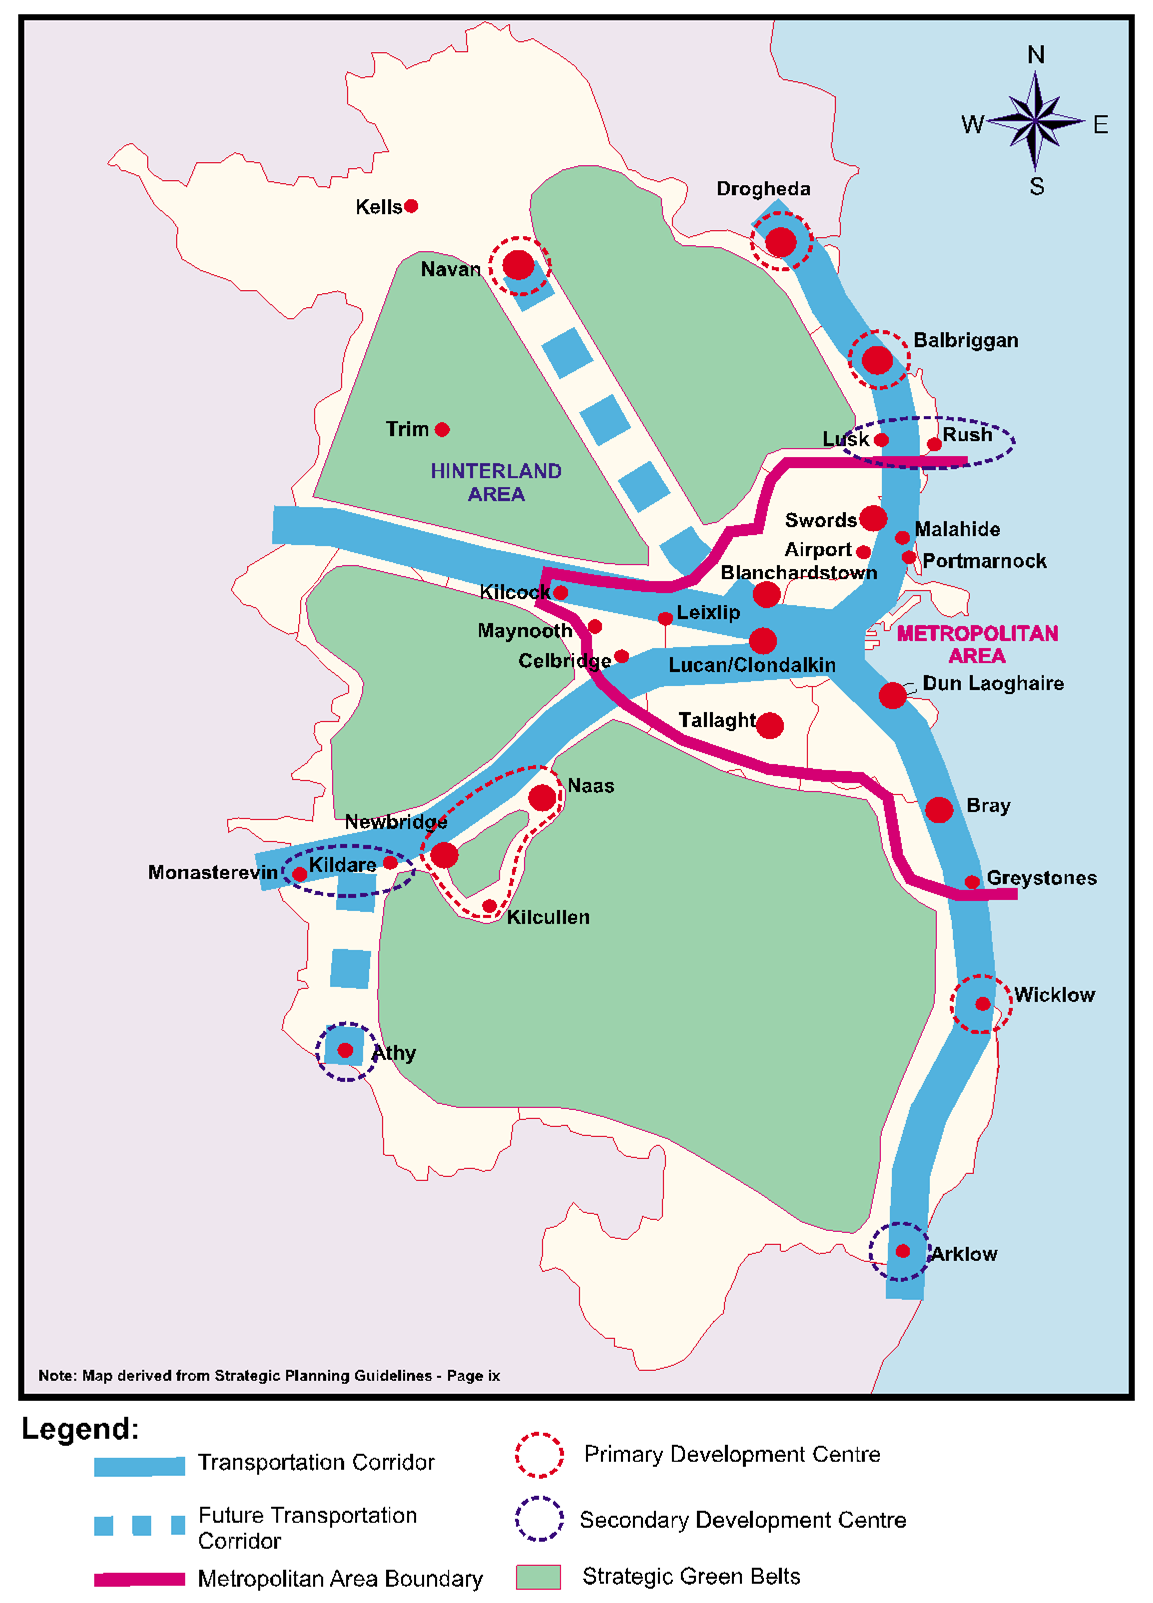
\includegraphics[width=\textwidth]{intro1.png}
\vfill

\section{More about the Introduction chapter}
The introduction allows you to orient the reader to your research project and
preview the organisation of your thesis. In the introduction, state what the
topic is about, explain why it needs to be further researched and introduce
your research question(s) or hypothesis.

Whilst patterns of organisation in introductions vary, there are some common
features that will help you to achieve an informative and engaging
introduction. Let’s identify these features:

\begin{itemize}
	\item Introduce the topic
	\item Define key terms and concepts
	\item Give background and context for the topic (this may include a brief literature
	      review)
	\item Review and evaluate the current state of knowledge in the topic (this may
	      include a brief literature review)
	\item Identify any gaps, shortcomings and problems in the research to date
	\item Introduce your research question(s) or hypothesis
	\item Briefly describe your methodology and/or theoretical approach
	\item Explain the aim of your research and what contribution it will make to the
	      topic
	\item Give an overview of the chapter outline of the thesis.
\end{itemize}

It’s important to note that, depending on your field of study and the faculty
requirements of your thesis, not all of these features will be relevant. Also,
these features may occur in varied orders.

Most people write many drafts of their introduction. It can be useful to write
one early in the research process to clarify your thinking. You will need to
write a version for your confirmation proposal and other milestones. As your
research progresses and your ideas develop, you will need to revise it. When
the final draft of chapters is complete, check the introduction once more to
make sure that it accurately reflects what you have actually done.
